\documentclass[tikz,border=15pt]{standalone}
\usepackage{tikz}
\usepackage{amsmath}
\usepackage{amsfonts}
\usetikzlibrary{arrows.meta,positioning,shapes,fit,backgrounds,calc}

\begin{document}
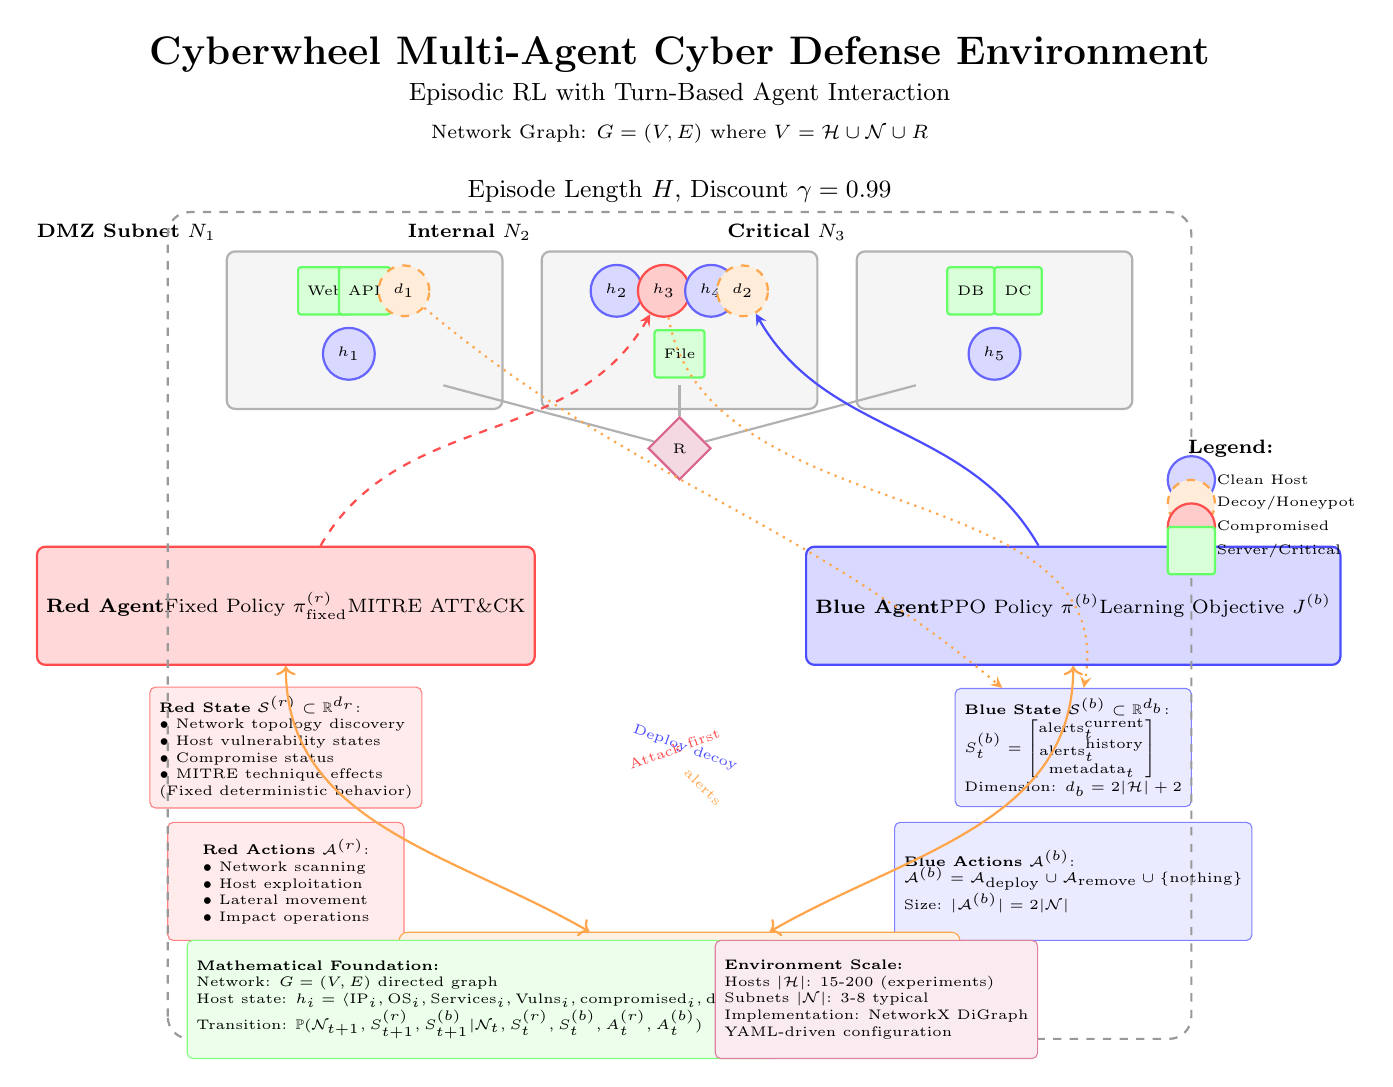
\begin{tikzpicture}[
    % Host and network styles
    host/.style={circle, draw=blue!60, fill=blue!15, minimum size=6mm, font=\tiny, thick},
    decoy/.style={circle, draw=orange!70, fill=orange!15, minimum size=6mm, font=\tiny, thick, dashed},
    compromised/.style={circle, draw=red!70, fill=red!20, minimum size=6mm, font=\tiny, thick},
    server/.style={rectangle, draw=green!60, fill=green!15, minimum size=6mm, font=\tiny, thick, rounded corners=1pt},
    subnet/.style={rectangle, draw=gray!60, fill=gray!8, minimum width=35mm, minimum height=20mm, font=\scriptsize, thick, rounded corners=3pt},
    router/.style={diamond, draw=purple!60, fill=purple!15, minimum size=8mm, font=\tiny, thick},
    % Agent styles  
    agent/.style={rectangle, draw=black, fill=yellow!15, minimum width=25mm, minimum height=15mm, font=\scriptsize, thick, rounded corners=3pt},
    % Info boxes
    statebox/.style={rectangle, draw=gray!50, fill=gray!5, rounded corners=2pt, font=\tiny, align=left, minimum width=30mm, minimum height=15mm},
    rewardbox/.style={rectangle, draw=orange!70, fill=orange!10, rounded corners=3pt, font=\tiny, align=center, minimum width=40mm, minimum height=12mm},
    % Arrows
    attack/.style={->, thick, red!70, dashed, >=stealth},
    defense/.style={->, thick, blue!70, >=stealth},
    alert/.style={->, thick, orange!70, dotted, >=stealth},
    flow/.style={->, thick, purple!60, >=stealth}
]

% Title
\node[font=\Large\bfseries] at (0, 9) {Cyberwheel Multi-Agent Cyber Defense Environment};
\node[font=\small] at (0, 8.5) {Episodic RL with Turn-Based Agent Interaction};

% Network Graph G = (V, E) representation
\node[font=\scriptsize] at (0, 8) {Network Graph: $G = (V, E)$ where $V = \mathcal{H} \cup \mathcal{N} \cup R$};

% DMZ Subnet (N1)
\node[subnet] (dmz) at (-4, 5.5) {};
\node[above left, font=\scriptsize] at (dmz.north west) {\textbf{DMZ Subnet} $N_1$};
\node[server] (web) at (-4.5, 6) {Web};
\node[server] (api) at (-4, 6) {API};
\node[decoy] (d1) at (-3.5, 6) {$d_1$};
\node[host] (h1) at (-4.2, 5.2) {$h_1$};

% Internal Subnet (N2) 
\node[subnet] (internal) at (0, 5.5) {};
\node[above left, font=\scriptsize] at (internal.north west) {\textbf{Internal} $N_2$};
\node[host] (h2) at (-0.8, 6) {$h_2$};
\node[compromised] (h3) at (-0.2, 6) {$h_3$};
\node[host] (h4) at (0.4, 6) {$h_4$};
\node[decoy] (d2) at (0.8, 6) {$d_2$};
\node[server] (file) at (0, 5.2) {File};

% Critical Assets Subnet (N3)
\node[subnet] (critical) at (4, 5.5) {};
\node[above left, font=\scriptsize] at (critical.north west) {\textbf{Critical} $N_3$};
\node[server] (db) at (3.7, 6) {DB};
\node[server] (dc) at (4.3, 6) {DC};
\node[host] (h5) at (4, 5.2) {$h_5$};

% Router (central network node)
\node[router] (router) at (0, 4) {R};

% Network backbone connections
\draw[thick, gray!60] (router) -- (-3, 4.8);
\draw[thick, gray!60] (router) -- (0, 4.8);
\draw[thick, gray!60] (router) -- (3, 4.8);

% Red Agent (Fixed Adversary)
\node[agent, fill=red!15, draw=red!70] (red_agent) at (-5, 2) {
    \textbf{Red Agent}\\
    Fixed Policy $\pi^{(r)}_{\text{fixed}}$\\
    MITRE ATT\&CK
};

% Blue Agent (Learnable PPO)
\node[agent, fill=blue!15, draw=blue!70] (blue_agent) at (5, 2) {
    \textbf{Blue Agent}\\
    PPO Policy $\pi^{(b)}$\\
    Learning Objective $J^{(b)}$
};

% Red Agent State Space
\node[statebox, draw=red!50, fill=red!8] (red_state) at (-5, 0.2) {
    \textbf{Red State} $\mathcal{S}^{(r)} \subset \mathbb{R}^{d_r}$:\\
    $\bullet$ Network topology discovery\\
    $\bullet$ Host vulnerability states\\
    $\bullet$ Compromise status\\
    $\bullet$ MITRE technique effects\\
    (Fixed deterministic behavior)
};

% Blue Agent State Space  
\node[statebox, draw=blue!50, fill=blue!8] (blue_state) at (5, 0.2) {
    \textbf{Blue State} $\mathcal{S}^{(b)} \subset \mathbb{R}^{d_b}$:\\
    $S_t^{(b)} = \begin{bmatrix} \text{alerts}_t^{\text{current}} \\ \text{alerts}_t^{\text{history}} \\ \text{metadata}_t \end{bmatrix}$\\
    Dimension: $d_b = 2|\mathcal{H}| + 2$
};

% Action Spaces
\node[statebox, draw=red!50, fill=red!8] (red_actions) at (-5, -1.5) {
    \textbf{Red Actions} $\mathcal{A}^{(r)}$:\\
    $\bullet$ Network scanning\\
    $\bullet$ Host exploitation  \\
    $\bullet$ Lateral movement\\
    $\bullet$ Impact operations
};

\node[statebox, draw=blue!50, fill=blue!8] (blue_actions) at (5, -1.5) {
    \textbf{Blue Actions} $\mathcal{A}^{(b)}$:\\
    $\mathcal{A}^{(b)} = \mathcal{A}_{\text{deploy}} \cup \mathcal{A}_{\text{remove}} \cup \{\text{nothing}\}$\\
    Size: $|\mathcal{A}^{(b)}| = 2|\mathcal{N}|$
};

% Turn-based interaction arrows
\draw[attack] (red_agent) to[out=60, in=240] (h3) node[midway, above, font=\tiny, rotate=20] {Attack first};
\draw[defense] (blue_agent) to[out=120, in=300] (d2) node[midway, above, font=\tiny, rotate=-20] {Deploy decoy};

% Alert flows (observation)
\draw[alert] (h3) to[out=280, in=80] (blue_state) node[midway, right, font=\tiny, rotate=-45] {alerts};
\draw[alert] (d1) to[out=320, in=140] (blue_state);

% Reward System (Adversarial)
\node[rewardbox] (rewards) at (0, -2.8) {
    \textbf{Adversarial Reward System}\\
    $R_t^{(b)} = \alpha_1 \cdot \text{deploy} + \alpha_2 \cdot D_t^{\text{decoy}} - \alpha_3 \cdot D_t^{\text{success}} - \alpha_4 \cdot \text{remove}$\\
    $R_t^{(r)} = \beta_1 \cdot D_t^{\text{success}} - \beta_2 \cdot D_t^{\text{decoy}}$\\
    Zero-sum: Deception $(+15, -5)$, Compromise $(-10, +10)$
};

% Reward connections
\draw[<->, orange!70, thick] (red_agent) to[out=270, in=150] (rewards);
\draw[<->, orange!70, thick] (blue_agent) to[out=270, in=30] (rewards);

% Environment boundary and episode info
\draw[thick, black!40, rounded corners=8pt, dashed] 
    (-6.5, -3.5) rectangle (6.5, 7);
\node[above, font=\small] at (0, 7) {Episode Length $H$, Discount $\gamma = 0.99$};

% Mathematical foundation
\node[statebox, draw=green!50, fill=green!8] (math) at (-2.5, -3) {
    \textbf{Mathematical Foundation:}\\
    Network: $G = (V, E)$ directed graph\\
    Host state: $h_i = \langle \text{IP}_i, \text{OS}_i, \text{Services}_i, \text{Vulns}_i, \text{compromised}_i, \text{decoy}_i \rangle$\\
    Transition: $\mathbb{P}(\mathcal{N}_{t+1}, S_{t+1}^{(r)}, S_{t+1}^{(b)} | \mathcal{N}_t, S_t^{(r)}, S_t^{(b)}, A_t^{(r)}, A_t^{(b)})$
};

% Scale info
\node[statebox, draw=purple!50, fill=purple!8] (scale) at (2.5, -3) {
    \textbf{Environment Scale:}\\
    Hosts $|\mathcal{H}|$: 15-200 (experiments)\\
    Subnets $|\mathcal{N}|$: 3-8 typical\\
    Implementation: NetworkX DiGraph\\
    YAML-driven configuration
};

% Legend
\node[font=\scriptsize] at (7, 4) {\textbf{Legend:}};
\node[host] at (6.5, 3.6) {}; \node[right, font=\tiny] at (6.7, 3.6) {Clean Host};
\node[decoy] at (6.5, 3.3) {}; \node[right, font=\tiny] at (6.7, 3.3) {Decoy/Honeypot};
\node[compromised] at (6.5, 3.0) {}; \node[right, font=\tiny] at (6.7, 3.0) {Compromised};
\node[server] at (6.5, 2.7) {}; \node[right, font=\tiny] at (6.7, 2.7) {Server/Critical};

\end{tikzpicture}
\end{document}